\chapter{Robot Design and Implementation}

% - Size and weight/energy availability/speed trade-off model and 
% - Should the subsections more or less reflect the columns in the table?
% - No optical encoders because they require a lot of energy!
% - Same for linefolower / mouse sensor.

\section{Design Requirements}
\label{sec:design_requirements}

% - Small form factor
% - Navigation
% - Power (should not rely on batteries)
% - However should be able to be powered from batteries for testing and tuning!
% - Tradeoff chargetime and operation time
% - Weight of the robot
% - Low voltage decreases power consumption of components and allows efficient use of the energy from the supercapacitor
% - Single mainboard design
% - Swarm robots are typically limited to only operate on flat surfaces!
% - Limited resources (no power hungry components ie optical encoders or mouse sensors)
% - Optimize or low power consumption (disable or standby sensors and motor ctrl when not used)

% RF harvesting seems prommesing
% better to only use RF for communication and harvest energy from another source \cite{konstantioulos}
% wispcam long time to charge

The main requirement for the robot is  that it should be battery-less, therefore it can only store a small amount of energy in a capacitor / small buffer.
Bigger capacitors have in general larger leakage currents.
As a result these require longer charge time

Size of the robot i.e weight and the required power for movement do not scale linearly.

To make efficient use of the energy stored in a supercapacitor a regular is required to supply a stable voltage to the connected loads.
The regulated output voltage is a lower threshold for the energy that can be used from the capacitor.
The upper threshold is typically determined by the maximum voltage rating of the supercapacitor.
Lowering the output voltage allows for more energy to be used from the supercapacitor, but also lowers the overall power consumption of individual components.
The energy stored in supercapacitor is a function of the capacitance and the threshold voltage difference, being equal to:

\begin{equation}
\label{eq:cap2}
E = \frac{1}{2}C(V_{max} - V_{min})^{2}
\end{equation}


	
\section{Hardware Implementation}

% - EXPLAIN MORE ABOUT HARDWARE CHOISES, why these specific componens. What were the requirements for choosing these components

The first step was to evaluate what components are required for the robot to have basic navigation capabilities.
Based on this, there was searched for commercially available low power components with the lowest minimal supply voltage.
Currently there are only a limited amount of motor controllers on the market that can operate at the 2.0V.
To make sure that a small drop in system voltage would not create instability a margin of 0.2V was added.
Now the system voltage of 2.2V has been determined, each part of the robot will be explained in more detail. 

\subsection{Computation and Sensing}

The robot is designed around a WISP 5 \cite{wisp5_wiki_2017}, a battery-free platform for low power sensing, computation and communication.
This platform has the ability to communicate with RFID readers and is powered by the carrier signal emitted by the reader.
However, the communication range and the power that can be harvested is limited.
Therefore communication is currently not implemented and a different energy source for harvesting will be used.
Currently only the microcontroller is being utilized, a Texas Instruments MSP430FR5969 ultra low power microcontroller.
This MCU can operate at 16 MHz and features 64 KB FRAM, 2 KB SRAM and 40 IO.

The robot has access to basic sensors which can be interfaced trough I2C.
For detecting obstacles in front of the robot, a Maxim Integrated MAX44000 proximity sensor was added of the robot facing forward.
This sensor switches a IR led at high frequency to reduce the power consumed.
The same sensor is based around a photo-diode it can be used to measure the amount of ambient light as well.
To allow for controlled movements the robot has a Bosch Sensortec BMG250 low power triaxial gyroscope to measure yaw-rate, used to correct it's heading when necessary.

\subsection{Locomotion}

% tell that also higher geared motors were tried??

Two dc motors with a 25:1 gearbox from Precision Microdrives are mounted in a 3d printed frame. %, directly under the mainboard of the IPR.
The motors are mounted diagonally opposite from each other making the robot as compact as possible, while this differential drive configuration allows the robot to steer.
Small plastic wheels with rubber tires are mounted directly on each of the motor shafts.
Behind these two motors a free running caster wheel is mounted to the frame, acting as a third support point for the robot.

The speed of each motor can be controlled individually using Pulse-Width-Modulation (PWM) and a Texas Instruments DRV8836 dual H-bridge.
Typically MCU io-ports are limited in the amount of current that they can supply.
MOSFETs inside the dual H-bridge allow regulation of larger currents to the motors.
The MCU can use the H-bridge to enable, disable and control the direction of rotation of each individual motor.

On average the each motor consumes 38mA while running on a flat surface, which is well within the current limit that the buck converter can supply.
However when the motors are in not moving yet the start current is approximately equal to the stall current, which is equal to 240mA.
This amount of current can not be supplied by a most regulators, PWM can be used to reduce the average current allowing a bulk capacitor to supply the voltage.

\subsection{Energy Harvesting}
\label{subsec:energy_harvesting}

Solar energy is harvested from two IXYS SLMD121H04L-ND solar cells in series.
These monocrystalline solar cells have a high efficiency of 22\%, allowing energy harvesting even in low light conditions.
The solar cells are connected to a Texas Instruments BQ25570 energy harvester. 
This harvester includes a nanopower boost charger with maximum power point tracking to extract the optimal amount of energy from the solar panel. 
The harvested energy is stored in a 22mF - 4.5V supercapacitor from AVX, chosen for it's low leakage current and small size.
The Texas Instruments BQ25570 has a buck converter to efficiently regulate the capacitor voltage down to the system voltage of 2.2V.
External resistors can be used to program voltage thresholds, allowing to automatically enable and disable the buck converter based on minimum and maximum thresholds.
Additionally the resistors are used to set the overvoltage protection and the buck converter output voltage.

\subsection{Integration}

% Check hardware section ivar
% Tell why pcb is required.
% Low power compontents have chip packages which are hard to solder by hand because of their small package size.
% More stability
% Tell about the Printed Circuit Board(PCB)

Now that all the parts have been chosen, they can be connected together to form the robot.
For ease of connection and because most parts come in small non-hand solderable packages, a Printed Circuit Board (PCB) has been designed, see Figure \ref{fig:pcb_robot}
Most reference designs are extendable but this adds complexity, while weight and size are the main constraints of this robot design.



\begin{figure}
	\centering
	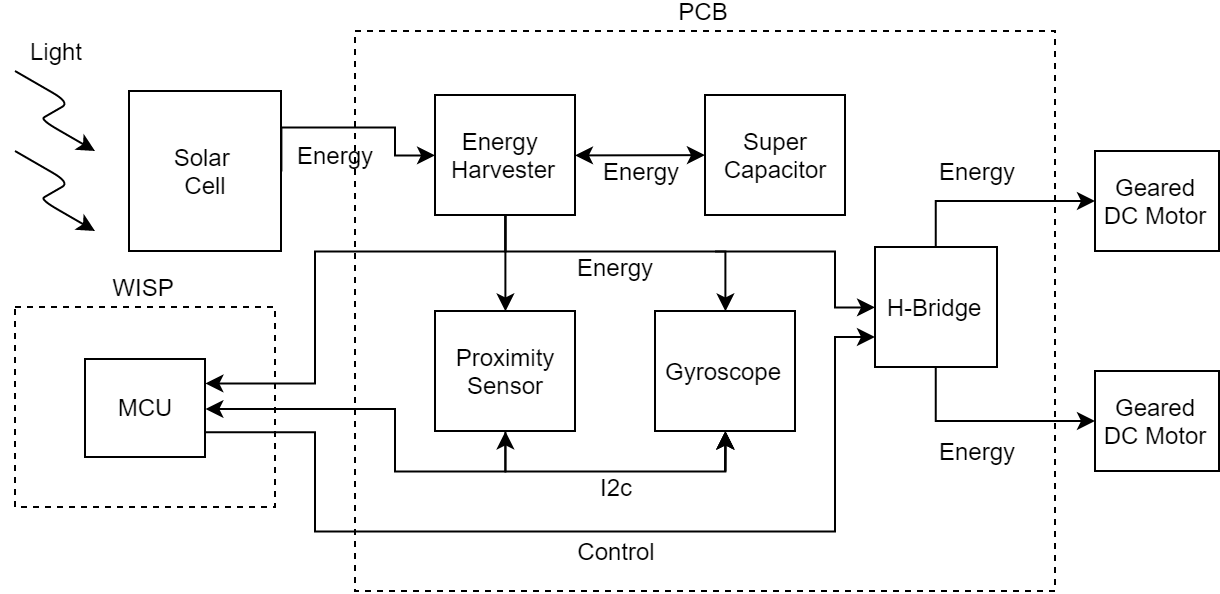
\includegraphics[width=\textwidth]{pics/schematic_robot_v2.png}
	\caption{Overview of a single robot}
	\label{fig:system_overview}
\end{figure}


\begin{figure}
	\centering
	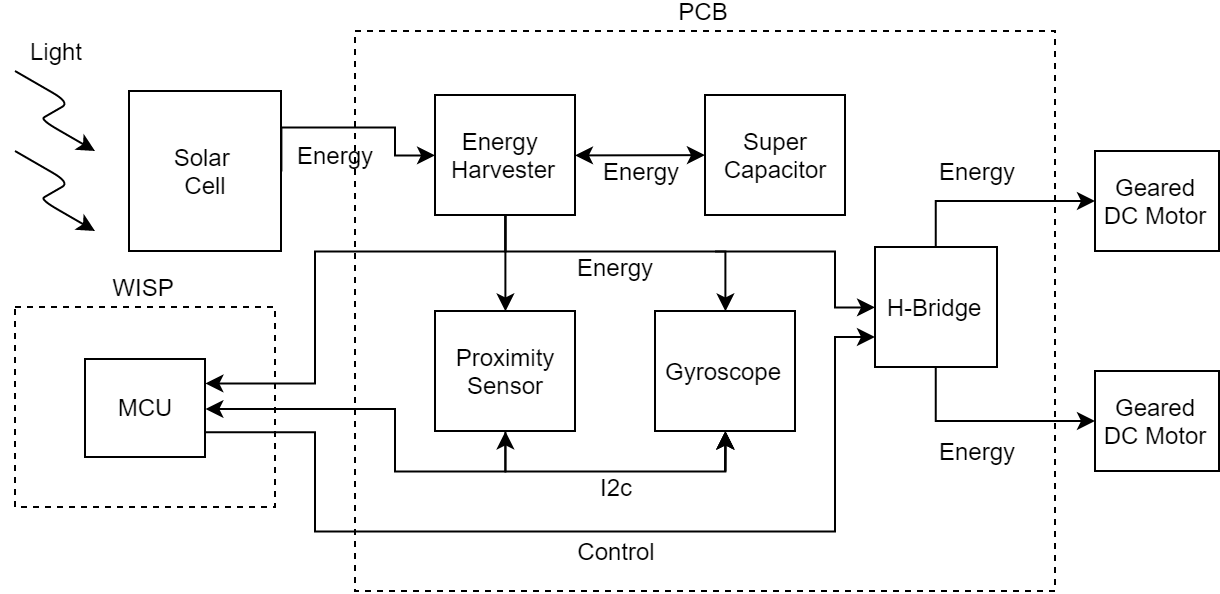
\includegraphics[width=\textwidth]{pics/schematic_robot_v2.png}
	\caption{PCB DESIGN}
	\label{fig:pcb_robot}
\end{figure}


% Make a overview of the cost to build a robot

\begin{table*}[t]
	\centering
	\caption{Power consumption of each individual component at 2.2V}
	\label{tab:1}
	\begin{tabular}{l l l} 
		\hline
		\\[-1em]
		Part & Active Current & Standby Current\\ 
		\hline
		\\[-1em]
		Proximity sensor & 432\textmu A & 0.1\textmu A \\
		Gyroscope & 650\textmu A & 3\textmu A\\	
		Microcontroller @ 8MHz & 1mA & N/A \\
		H-bridge & 1.2mA & 10nA \\
		DC motor & 39mA & N/A \\
		DC motor & 39mA & N/A \\
		\hline
		\\[-1em]
		Total & xx & xx \\
	\end{tabular}
\end{table*}


\section{Software Implementation}

% General library for reading and writing to i2c.

% How program consistency (ie progress) is maintained given the intermittend nature of the robot.

% A operating system for intermittend devices

\subsection{Calibration of the motors}
\label{subsub:motor_calib}

% Write about why valid to assume a constant speed on a single surface
In robotics the motors are commonly powered directly from the battery as linear or switch-mode power regulators are not able to supply the high start-up currents.
When the motors are powered from the battery the supplied voltages drops while energy is consumed for the battery.
Since the speed of the motor is dependent on the supply voltage the speed of the motor will also decrease while energy is consumed from the battery.
However, the use of a supercapacitor requires a regulator to make efficient use of the energy stored, as described in Section \ref{subsec:energy_harvesting}.
A benefit of running a constant voltage is that the supply voltage is not a factor anymore which can change the motor speed.
NEED MORE EXPLANATION
By making the assumption that the robot will only travel on a flat surface, the speed is considered constant given a certain PWM duty-cycle.


\subsubsection{PWM frequency for linear motion control}
% Write about linear motion control dc motor vs pwm
% Reference: https://www.precisionmicrodrives.com/application-notes/ab-022-pwm-frequency-for-linear-motion-control

Pulse width modulation(PWM) is used to control the speed of the motors, by changing the duty cycle of the control pulse the average current through the motors can be changed.
The winding current is proportional to the torgue output of the motor and therefore the average winding current is proportional to the PWM duty cycle.
However this is only true for pure resistive loads,

%Typically operation frequency is above 20 khz (what people can hear)

% -Write how the pwm control signals are generated for the H-bridge. 
The PWM signals are generated by the microcontroller on the WISP.
Luckily four io-ports are available on the WISP which can be directly controlled by a single timer running at 2kHz.
The timer is configured to use a compare register for each of the ports.
When the timer reaches a value that corresponds to a value one of the compare registers the connected port is toggled automatically.
This way the overhead is minimized because no interrupt service routine is required.

\subsubsection{Duty cycle selection}

The next step is to determine the minimum and maximum PWM duty-cycle that will enable the motor to turn.
A minimal PWM duty-cycle to produce a torque that is able to overcome the static friction between the wheels and a surface the robot is moving on.
Each motor is physically different and the friction in the gearbox can variate as well, which results in a different output speed per motor.
Since the robot uses two motors in differential drive configuration, a minimum PWM duty-cycle has to be found for each motor.
This is accomplished by setting a PWM duty-cycle at which both motors are rotating and slowly backing down the PWM duty-cycle until one or both stop turning.
The minimum PWM duty-cycle, allowing the wheels to rotate, is then saved and added to every motor set point.
If the robot is commanded to run at this minimum speed it will be very likely that it will not yet travel in a straight line.

% -Write about maximum speed due to enabling two motors and their startup current peak! show figure!!
% -Write about current generated by the lack of Back-EMF
% -Use large capacitor to somewhat reduce the effect! NEED FIGURE!
%TODO -Write about bounding the pid output, because otherwise the motors of the robot could stall, if the motor setpoint is to high
% Does more gearing (more torque) reduce the current peak??
% How does pwm influcence the startup current of the motor in combination with a capacitor
% The pwm frequency seems to have a effect as well; higher freq preforms better??
% Maybe something with RC TIME?

The maximum PWM duty-cycle is bounded by the amount of current that the buck converter and bulk capacitor can supply.
Lowering the PWM duty-cycle can reduce the current peak induced by the lack of back-EMF when the motor is in steady state.
When the set point is just to high a kind of clicking noise can be heard, indicating that the start current peak of motor is to high and the power supply is not able to supply the current.


\begin{equation}
\frac{dV}{dt} = \frac{I}{C}
\end{equation}

Allow 0.2V voltage drop (msp430 and motor driver stop working)

% DO calculation of current that can be supplied from capacitor buffer

 


\subsection{Closed loop feedback for controlled movements}

The robot uses two physically different motors in differential drive configuration which are mounted in a non-symmetrical way.
Open loop movement using just a calibrated motor values has been used in previous work \cite{legoc_uist_2016}, but it can be time consuming and any little disturbance will trow the robot off course.
The gyroscope is used to obtain the current yaw-rate and correct the robots heading.
Controlled movements are possible using closed loop feedback, where the heading is used to update the motor control values.

The robot can be controlled using three different commands, one for straight trajectories, one for left and one for right turns.
When a command is executed a control loop will run until the provided target is reached.
A timer running periodically calling a interrupt service routine which executes the control loop.   
Each command requires different initial values, set points and tuning parameters, these are set accordingly before the control loop is enabled.

\subsubsection{Controlled straight trajectories}

% -Why pid for straight movements and not a simple p controller?
% --Fast reaction on disturbances without osccilation??

The control loop for straight trajectories obtains the yaw-rate from the gyroscope and uses this as an input for the Proportional–Integral–Derivative (PID) controller.
The PID will try to reduce the error and force the yaw-rate to zero for a given target motor speed.
% $ e(t) = 0 - yaw(t)$
Using the output of the PID controller the target motor speed of each motor is adjusted in opposite direction.
The loop will stop automatically when the required target is reached.
%TODO Explain that the target distance is with a calibrated value.

\begin{equation}
output(t) = K_{p}e(t) + K_{i} \int_{0}^{t}e(\tau)d\tau + Kd\frac{d}{dt}e(t) [rad/s]
\end{equation}

\subsubsection{PID tuning using Ziegler-Nichols method}

%TODO -Write about tuning the pid controller using Ziegler–Nichols tuning method (method 2), closed loop, Critical gain.

A PID loop can be tuned using three different tunable gains ($K_{p}$, $K_{i}$, $K_{d}$).
Tuning can be done trough a trail and error approach but a faster way of tuning is to use the Zigeler-Nicholos method.
The second or ultimate gain method starts with increasing or decreasing Kp until constant oscillation occurs.
From Figure \ref{fig:ultimate_gain} can be seen how the proportional gain was increased until eventually the robot started to oscillate.
With a proportional gain of 0.13 the robot starts light oscillation at the end, but this is not always the case and can be a result of the surface the robot was driving on.
% Tell something about how the right values are determined
To reduce the oscillation a $T_{u}$ of 0.2 was added as can be determined from Figure \ref{fig:gain_tuning}.
From this figure can be seen that the robot is more stable and doesn't have the intension to oscillate anymore.
Robots was driving on surface that was not super flat, therefore the gyro signal is noisy.
The tuning process was sped up by setting the minimum motor duty-cycle as it made the robot a lot more responsive, this was described earlier in Section \ref{subsub:motor_calib}.

%TODO -Add figure with critcial gain + mark period Tu

\begin{figure}[!tbp]
	\begin{subfigure}[b]{0.5\textwidth}
		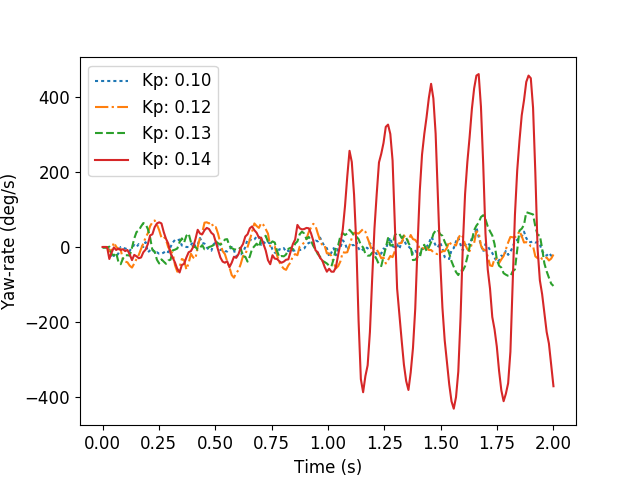
\includegraphics[width=\textwidth]{pics/straight_ku.png}
		\caption{Increase Ku until oscillation}
		\label{fig:ultimate_gain}
	\end{subfigure}
	\begin{subfigure}[b]{0.5\textwidth}
		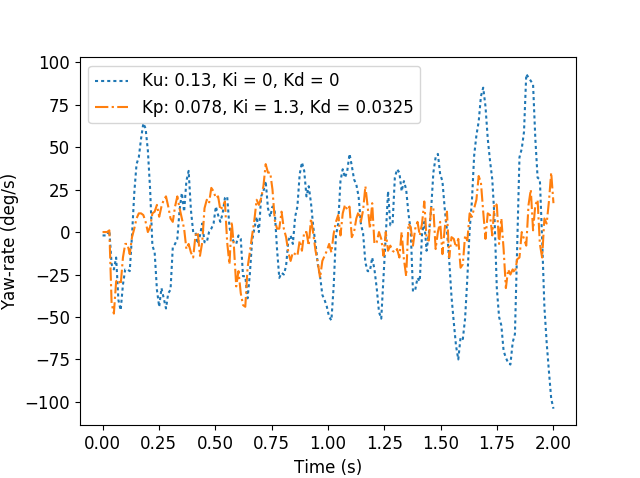
\includegraphics[width=\textwidth]{pics/straight_ku_with_tu.png}
		\caption{Find period}
		\label{fig:gain_tuning}
	\end{subfigure}
	\caption{Tuning the PID controller using the ultimate gain method}
\end{figure}

\subsubsection{Controlled turns}

The control loop for controlled turning uses the angle, which can be obtained by integrating the yaw-rate sensor data from the gyroscope.
A P controller is used to rotate the robot to the desired angle, the proportional gain is directly influencing turn speed of the robot.
The motor control values are set to run the motors opposite directions and are equal to the output of the P controller.
These values will keep decreasing until the robot rotates to the desired angle.
The set point is assumed to be reached when the angle is within two degrees of the target, in this case the loop will stop automatically.
To allow enough precision to be able to measure if the target is within these two degrees, the timer which executes the control loop was set to run at 100Hz.
Secondly, the proportional gain should not be set to low because it can happen that the robot is not able to reach the target but also not to high as it can overshoot the target.

\subsection{Persistent movement}

% Checkpointing / State keeping

% Dubble buffering for updating multiple dependent variables (keep consistency)